\chapter{Vorgehen}

\section{Inbetriebnahme des Modells der Machbarkeitsstudie}
Mit der in der Projektarbeit entwickelten Harvesterschaltung kann per Bluetooth Smart auf dem Android-Endgerät die Geschwindigkeit ausgegeben werden.
Bei der Inbetriebnahme zeigten sich folgende Grenzen im gegebenen Modell:

\begin{enumerate}
    \item Zu hoher Kondensator vor Energiemanagmenetschaltung gefährdet deren Stabilität
    \item Konfiguration auf Energiemanagementboard sind nicht auf Energieharvesterschaltung angepasst
\end{enumerate}


\subsection{Kapazität für Harvesting-Schaltung verbessern}

In der Machbarkeitsstudie ist nach dem Gleichrichter ein Kondensator von 470 $\mu$F nachgeschaltet. Dieser glättet die Spannungspulse nach dem Gleichrichter zu einer DC-ähnlichen Spannung mit Rippeln.

Mit einem Kondensator von 470 $\mu$F wird die Ausgangsspannung der Harvesterspannung fast rippelfrei. Die Rippelspannung beträgt 3.2 mV (siehe Abbildung \ref{kond470uF}).

\begin{figure}
    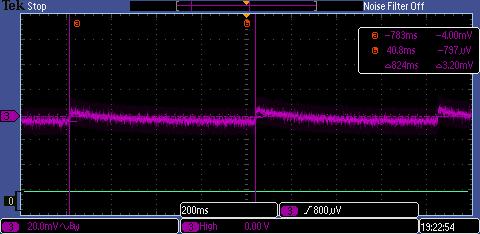
\includegraphics[width=15cm]{3Vorgehen/imag/470uF.PNG}
    \caption{Rippelspannung bei Glättung mit 470 $\mu$F Kondensator}\label{kond470uF} 
\end{figure}

Gemäss Ives \textbf{XXXXXX} von EM Microelectronics sollten Kondensatoren der Harvesterschaltung im Bereich von 4.7 $\mu$F liegen, sodass die Energiemanagementschaltung ordnungsgemäss funktioniert.  

Aus diesem Grund wird die Rippelspannung am Ausgangs der Harvesterschaltung mit kleineren Kondensatoren gemessen. Das Messprotokoll befindet sich im Anhang.

\subsubsection*{Messaufbau}
In der gegebenen Harvesterschaltung wird am Kondensator die Spannung mit einem Kathodenstrahloszilloskop (KO) gemesssen. Ausgehend vom bestehenden Kondensator (470 $ \mu $F), werden danach Elektrolytkondensatoren (Elko) mit den Werten 100 $\mu F $F, 47 $\mu$F und 10 $\mu$F gemessen.

\begin{figure}[h]
    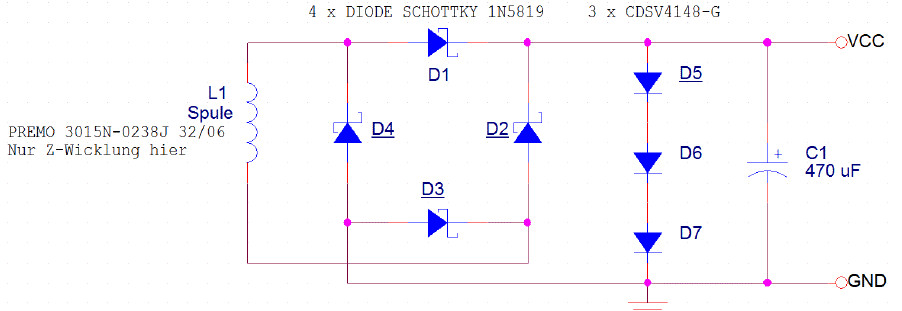
\includegraphics[width=15cm]{3Vorgehen/imag/messschaltungHarvesterschaltung.jpg}
    \caption{Messschaltung}
\end{figure}

\subsubsection*{Resultat}

Die Rippelspannung erhöht sich wie erwartet. Vpp beträgt bei 100 uF \textbf{xx} mV, bei 47 uF 28.8 mV (siehe Abbildung \ref{kond47uF}) und bei 10 uF 320 mV (Abbildung \ref{kond10uF}).
 
\begin{figure}
    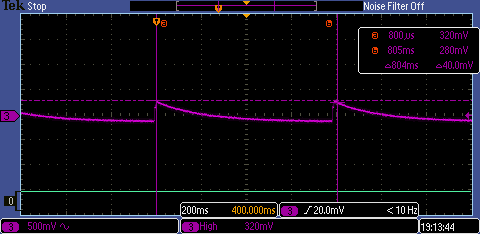
\includegraphics[width=15cm]{3Vorgehen/imag/10uF.PNG}
    \caption{Rippelspannung mit 10 uF Kondensator}\label{kond10uF} 
\end{figure}

\begin{figure}
    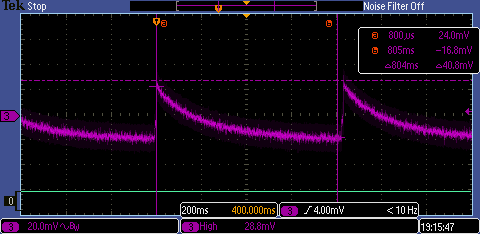
\includegraphics[width=15cm]{3Vorgehen/imag/47uF.PNG}
    \caption{Rippelspannung mit 47 uFKondensator}\label{kond47uF} 
\end{figure}


\subsubsection{Messungen Energy Management Board}
In der Projektarbeit findet sich auf S. 36 folgende Abbildung \ref{spannungMachbarkeit} zu den Spannungswerten des Modells der Machbarkeitsstudie.

\begin{tabbing}
    Channel\quad\= Farbe\quad\= Beschreibung\\[0.8ex]
    CH1\> gelb\> Spannung von Harvesterquelle\\
    CH2\> blau\> Spannung am STS--Kondensator\\
    CH3\> violet\> Spannung am LTS--Kondensator\\
    CH4\> grün\> Ausgangsspannung Energiemanagment\\
\end{tabbing}

\begin{figure}
    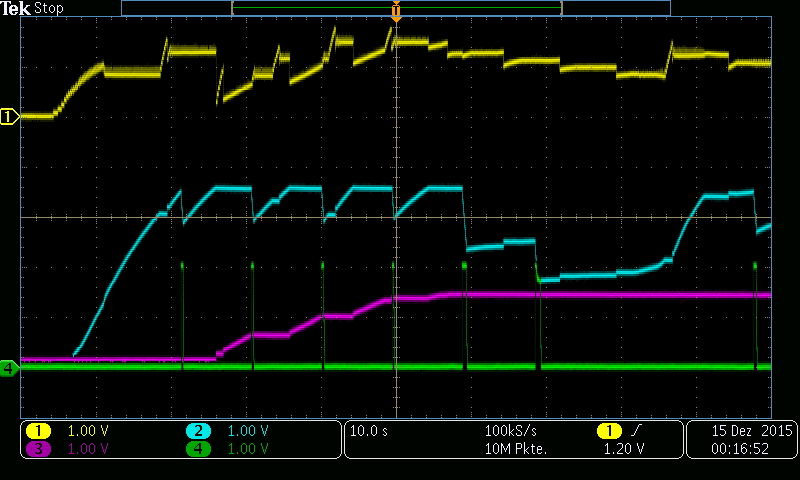
\includegraphics[width=15cm]{3Vorgehen/imag/messungPA.png}
    \caption{Spannungswerte Modell der Machbarkeitsstudie}\label{spannungMachbarkeit} 
\end{figure}

Auffällig sind zwei Spannungskurven: Die Spannung des Energieerzeugers. Die Spannungsregelung am Eingang der EMS funktioniert nicht korrekt. Zwischen zwei Regelperioden sollten konstante Spannungen eintreffen (siehe Erklärung in ref). 
Es zeigt sich, dass der LTS nicht geladen wird . Und es zeigt sich, dass das EM-Board nicht zu regulieren beginnt. Damit das Energiemanagement funktioniert, muss der Wer XXXX erreicht werden. Da dieser Wert nicht erreicht wird, passt die Energiemanagementschaltung den Innenwiderstand nicht auf.

Zum korrekten Einstellen des Energiemanagements braucht es eine MaximumPowerPointTracking-Ratio.



%--------------------------------------------------------------------------

\section{Layout Print}

Ein wichtiger Punkt der Arbeit ist die Miniaturisierung der bestehenden Hardware, das heisst der Aufbau aus der Machbarkeitsstudie soll auf eine Leiterplatte gebracht werden. Die Leiterplatte hat einige Vorgaben, welche im besten Fall alle eingehalten werden sollen.

\begin{enumerate}
    \item Die Leiterplatte soll nicht oder nur geringfügig grösser sein als das TI-SensorTag.
    
    \item Alle Netze sollen mit Testpunkten ausgestattet werden.
    
    \item Alle Anschlüsse vom TI-SensorTag sollen auf der Leiterplatte mit Testpunkten ausgestattet werden.
    
    \item Alle Testpunkte vom TI-SensorTag sollen in einem Raster von 2.54 mm angeordnet werden, damit ein Stecker kontaktiert werden kann.
    
\end{enumerate}
	


\subsection{Das Schema (oder der Stromlaufplan)}
Als erstes musste ein Schema, auch Stromlaufplan genannt, gezeichnet werden. Das Schema wurde Blockweise erfasst, als erstes wurde die Harvesterschaltung erfasst. Das Schema wurde aus der Machbarkeitsstudie entnommen. Die Funktionsweise der Harvesterschaltung kann wieder in mehrere Teile unterteilt werden.

\begin{enumerate}
    \item Die Spule: Gewinnt Energie aus dem vorbei schnellenden Magneten.
    
    \item Der Gleichrichter: Erzeugt positive Pulse aus der induzierten Spannung.
    
    \item Der Limiter: Limitiert die Spannung auf eine fixe Spannung.
    
    \item Der Ausgangskondensator: Glättet die positiven Pulse aus dem Gleichrichter.
    
\end{enumerate}

Der nächste Block ist der EM8500-Chip mit seinen Stützkondensatoren. Das Schema wurde aus dem Datenblatt entnommen. 
Die Energiespeicher, welche in dieser Arbeit mittels Elektrolytkondensatoren dargestellt werden, sind einige der wichtigsten Elemente. Die Speicherelemente werden nicht auf der Leiterplatte Platz finden, da die meisten Elektrolytkondensatoren zu hoch sind und der Platz zwischen den Leiterplatten sehr gering ist. 
Die Umlauferfassung wird mit einem Reed-Switch ermöglicht. Der Reedswitch ist einer der kleinsten Blöcke im Schema.
Der Block Interface enthält die Verbindung zum TI-SensorTag, ein Stecker realisiert dieses Interface. Der Stecker ist bereits vom TI-SensorTag vorgegeben, es handelt sich um einen Stecker, welcher sein eigenes Gegenstück darstellt. 

\subsection{Optimierung der Harvesterschaltung}
% Zwei Gründe:
- Ives: Der Glättungskondensator wird auf 47 uF geändert. 
- Zu wenig Energie für 10 km/h

Nach dem Erfassen des Schemas wurde die Optimierung der Hardware angegangen. Die beste Optimierungsmöglichkeit und auch der kritischste Block ist die Harvesterschaltung, hier wird die Energie für die restliche Schaltung gewonnen. In mehreren Schritten wurden die einzelnen Teile der Schaltung analysiert und versucht zu optimieren.

\subsubsection{Optimierung der Spule}

Die Spule gewinnt die Energie aus dem vorbei schnellenden Magneten, hier kann die gewonnene Energie beeinflusst werden. Eine gute Spule kann mehr Energie aus dem bewegten Magneten gewinnen, wichtig ist die Induktivität L und die Fläche A, welche die Spule hat. Eine Vorgabe war dass die Spule von der Grösse nicht merklich verändert wird, ausser man würde eine kleinere Spule finden, welche mehr Energie gewinnt. Eine Spule mit ähnlicher Fläche bzw. Grösse wurde gefunden, welche eine höhere Induktivität besitzt. Die Spule von Würth Elektronik ist sehr vielversprechend, denn die gleiche Fläche mit höherer Induktivität bedeutet mehr Energiegewinn aus dem Magneten.
Hier Schlusswort von Messprotokoll einfügen.

\subsubsection{Optimierung des Gleichrichters}

Der Gleichrichter aus dem Aufbau der Machbarkeitsstudie besteht aus vier Dioden vom Typ 1N5819, diese Dioden sind nicht für eine LowPower-Anwendung ausgelegt. Ausserdem könnte ein Gleichrichter gefunden werden, welcher in einem Gehäuse ausgeliefert wird. Wichtig ist dass der Leckstrom so gering wie möglich ist und die Schwellenspannung ebenfalls möglichst klein bleibt. 
Hier Schlusswort vom Messprotokoll einfügen.

\subsubsection{Optimierung des Limiter}

Der Limiter ist eine Spannungbegrenzung, da die nachfolgende Schaltung nicht mit einer zu hohen Spannung betrieben werden darf. Dieser Schaltungsteil ist sehr kritisch, denn er darf nicht zu viel Energie verlieren, muss aber trotzdem die Spannung immer begrenzen. Die Spannung darf einen Pegel von 2 V nicht überschreiten, da ansonsten der EM-8500-Chip droht zerstört zu werden. 
Hier Schlusswort vom Messprotokoll einfügen.

\subsubsection{Optimierung des Ausgangskondensators}

Der Ausgangskondensator muss möglichst niedrig gehalten werden, gemäss Aussage von Yves, da ansonsten der EM8500-Chip Mühe hat den Eingang zu regeln. Trotzdem darf der Ausgangskondensator nicht zu klein dimensioniert werden, da ansonsten die Rippelspannung am Ausgang der Harvestersschaltung zu hoch ist und der EM8500-Chip ebenfalls nicht mehr richtig regeln kann.
Hier Schlussword vom Messprotokoll einfügen.


\subsection{Bauteildefinition}

Nachdem das Schema gezeichnet wurde und die Schaltung opimiert wurde, mussten die Bauteile noch definiert werden. Es mussten die Footprints, sowie die Hersteller, Herstellerbezeichnungen, Lieferant und Lieferantenartikelnummer hinterlegt werden. Einige Footprints waren bereits in den Bibliotheken vorhanden, welche wir von Lukas erhalten haben. Fehlende Footprints wurden ergänzt, wie zum Beispiel der Footprint der Spule.


\subsection{Das Layout}

\subsubsection{Positionierung}
Die Positionierung der Bauteile auf der Leiterplatte ist sehr wichtig, da hier schon unnötige Leiterbahnen gespart werden können bzw. die Länge von gewissen Leiterbahnen können extrem verkürzt werden.
Wichtig ist, dass die Stüztkondensatoren bei dem EM8500-Chip so nah wie möglich am Chip platziert werden, damit die Spannungen am Chip so konstant gehalten werden können, wie nur möglich.
Weiter sollte die Harvesterschaltung ebenfalls sehr eng beieinander platziert werden, um zu verhindern, dass durch lange Stromlaufwege bereits Leistung verloren geht. Problematisch ist, dass die Spule auf der unteren Seite der Leiterplatte platziert werden muss, somit wird die Schaltung ein auf zwei Layer aufgeteilt.
Eine grosse Herausforderung ist die Positionierung der Testpunkte, um das Interface zum TI-SensorTag zu realisieren. Dadurch wird ein grosser Platz für die korrekte Positionierung der Testpunkte eingenommen.

\subsubsection{Gestaltung der Leiterbahnen}

Wann immer möglich wurden die Leiterbahnen, welche zu der Harvesterschaltung gehören, mit 20 Mil gezogen, um eine möglichst verlustfreie Leistungsübertragung zu gewährleisten. Alle anderen nicht leistungskritischen Leiterbahnen wurden mit eine Leiterbahnbreite von 10 Mil platziert, um nicht mehr Platz in Anspruch zu nehmen als nötig.

\subsubsection{Ergebnis}

Das Ergebnis ist eine Leiterplatte, welche alle gewünschten Spezifikationen erfüllt und somit kann die Leiterplatte auch für ein Praktikum verwendet werden. Die Leiterplatte ist mit sehr vielen Testpunkten ausgestattet, sowie die Möglichkeit für Strommessungen.

%--------------------------------------------------------------------------

\subsection{Energiekalkulation}
EHRV gesammelt >= BLESenden
Zeitkomponente
Energie Harvester braucht länger, verbrauch schneller.

Die Energie der Quelle [$\bar{E_{HRV}} $] muss ausreichen für das Versenden der Datenpakte über Bluetooth smart [$\bar{E_{BLE}}$].

\[\bar{E_{HRV}} \ge \bar{E_{BLE}}  \]


Die durchschnittliche maximale Leistung der Quelle kann aus der Abbildung \ref{MPP_Werte} entnommen werden. Diese basiert auf dem Messprotokoll im Anhang \ref{anhang_messprotokoll_energie_harvester}. 

MAN KÖNNTE. (GEHRÖT ZU OPTIONAL) Da die produzierter Energie von der Fahrgeschwindigkeit abhängt, wird das Energie-System in drei Zustände eingeteilt:

\begin{itemize}
    \item tiefe Geschwindigkeit: 0 - 10 km/h
    \item mittlere Geschwindigkeit: 10 - 20 km/h 
    \item hohe Geschwindigkeit: grösser als 20 km/h 
\end{itemize}



\subsubsection*{Leistungsabgabe Harvester-Schaltung}

\begin{tabular}{|l|l|}\hline \label{MPP_Werte} 
    Geschwindigkeit [km/h] & Maximale Leistung [$\mu W$] \\ \hline
    10 & 74.4 \\ \hline
    20 & unbekannt \\ \hline
    40 & unbekannt \\ \hline
\end{tabular}


Der Energieverbrauch hängt von der Anzahl ausgelesener Daten ab. Wird nur die Geschwindigkeit übermittelt, ist der Verbrauch kleiner, als wenn zusätzlich die Temperatur und die Höhe mitgesendet werden.


\subsubsection{MPP einstellen}
MPP:
- start bei 50 \% (wir bei 40), und grobe Schritte (unten . direkt auf 60 \%, dann 67 \%). 



\subsubsection*{Energieverbrauch BLE-Packete versenden}
 
\begin{tabular}{|l|l|}\hline \label{Energie_Pakete_Werte} 
    Anzahl Inhalte  & Energieverbrauch [$\mu J$] \\ \hline
    1 & 11000 \\ \hline
    2 & unbekannt \\ \hline
    3 & unbekannt \\ \hline
\end{tabular}

(Für die Zuverlässigkeit der Datenübermittlung wird jeweils dasselbe Paket über drei Kanäle gesendet. Wenn hier \glqq 1 Inhalt versenden \grqq  steht, meint dies, ein Paket über drei Kanäle senden.)

\subsubsection*{Berechnung}

\[\bar{E_{HRV}} = \bar{P} * t \ge \bar{E_{BLE}}  \]
\[\bar{P_{10km/h}} * t = 11 * 10^{-3}  \]
\[74.4 * 10^{-6} * t = 11 * 10^{-3}   \]
\[t = 147 s  \]

\[\bar{E_{HRV}} = \bar{P} * t \ge \bar{E_{BLE}}  \]
\[\bar{P_{10km/h}} * t = 11 * 10^{-3}  \]
\[74.4 * 10^{-6} * t = 11 * 10^{-3}   \]
\[t = 147 s  \]

\subsubsection*{EM BOARD KONZEPT}
Funktion generell beschreiben (im Anhang) 
\subsubsection*{Schwellwerte}
Ausrechnend der schwellwerte
\subsubsection*{Konfigurationen}
Konfigurationseinstellungen



\section{Low Power Einstellungen Sensortag}

Problem: So gehört zu jedem Aufwecken einer Peripherie, der Parallele Schlafmodus, bis dass die Peripherie gestartet ist. (Dies gilt auch für die Sensoren.) Zu lange warten: braucht Energie.

Sleep konkret: Power Banks abschalten:
Power Domains zeigen

Schwierigkeit Interrupt and Events !!

Gearbeitet wird mit einem Cortex M3 von TI. 
Grundsätzlich basieren die Bsp. auf RTOS. Wenige für PowerManagement. Das Powermanagement ohne Betriessystem. Wir verwenden dies, weil (gemäss Erfahrungswerte Praxis) mit Betriebsystem mehr Energie braucht).

\subsection{VO: SimpleBroadcast}
Ablaufdiagramm Senden
- Was ist der Unterschied zum RTOS.
- Was muss gemacht werden.

- Was überprüft werden musste, was gut ist.

Gestartet mit simpleBLE-Projekt von TI mit Einstellungen von Assistenten vom Ines.

\begin{figure}
  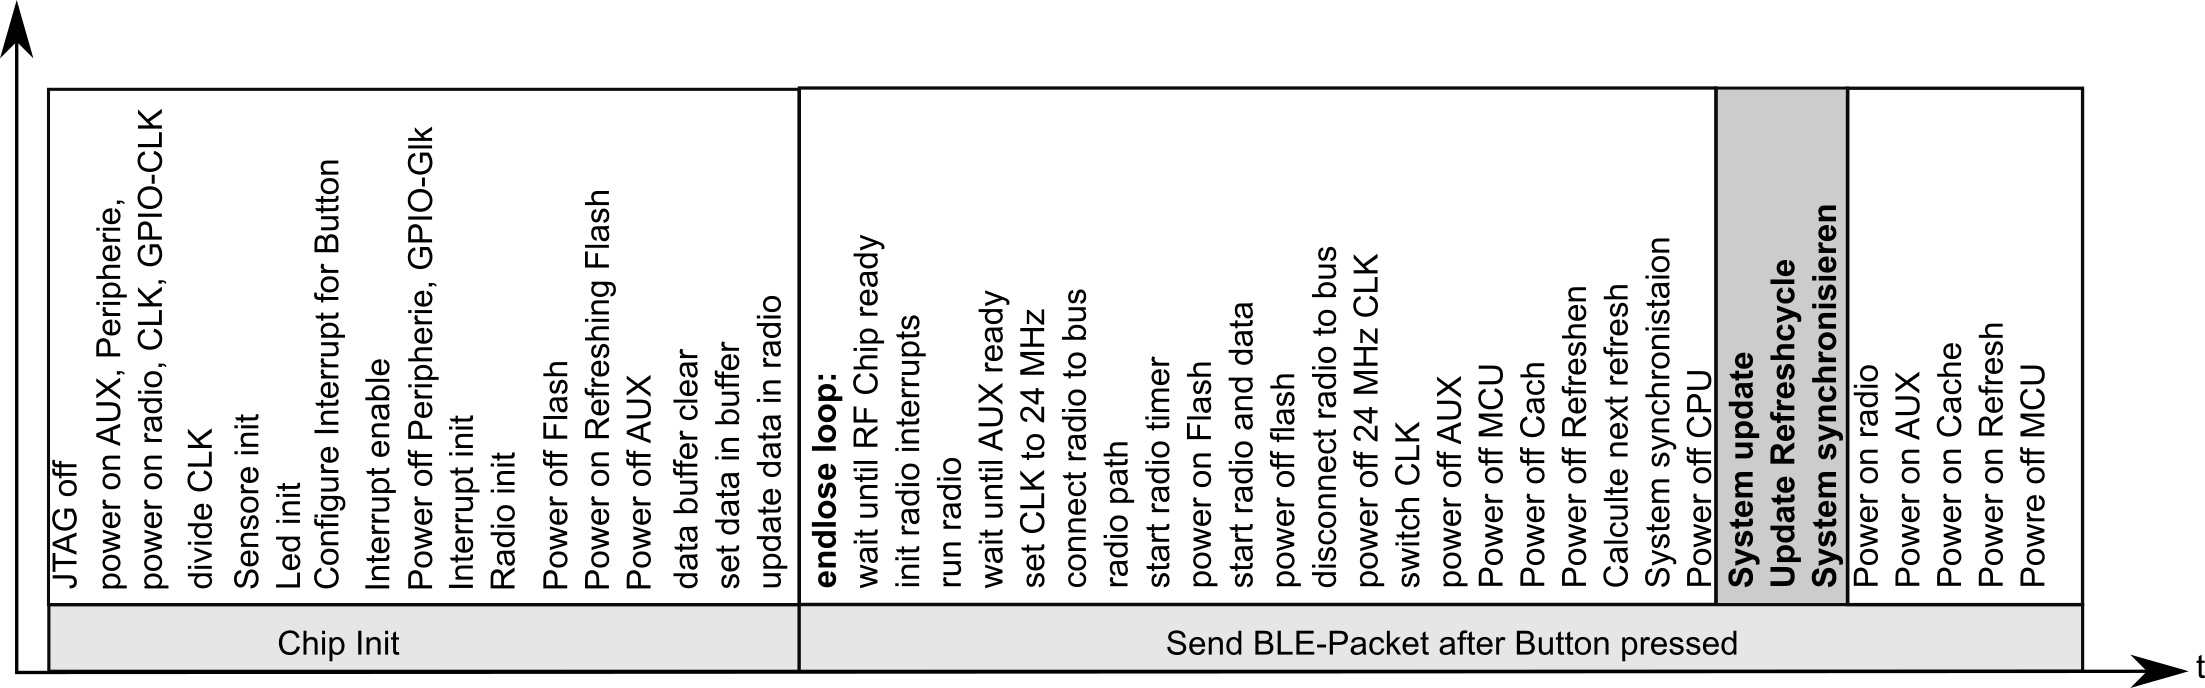
\includegraphics[width=15cm]{../ressources/SimpleLink/V0Sendeablauf.png}
  \caption{Prozessablauf V0}
\end{figure}




\begin{itemize}
    \item Configure ccfg.c to use internal LF RCOSC
    \item Configure WAKE INTERVAL
    \item Configure recharge period to 400ms if WAKE INTERVAL is larger than 400ms(ish)
    \item Configure IO's and set up advertisment payload       
\end{itemize}

Allgemeine Einstellungen in der Konfigurationsdatei ccfg.c:
Vmin = 2.25 V
Imax = 39 mA


Da VSUP bei 1.8 V startet, ist zu überprüfen. 


// RTC wakeup interval
\#define WAKE\_INTERVAL\_MS 		1000
\#define WAKE\_INTERVAL\_TICKS 	WAKE\_INTERVAL\_MS*65536 / 1000


// Advertisment payload length in bytes
\#define ADVLEN 10


Gehen in den Standby modus. Wird eingestellt über die Datei pwr\_ctr.c /h

Dort stehen alle Handlungen, die das System macht, um in den Standby-Modus zu gelangen.

\subsection{V1}


\subsection{V2}


\section{Applikationsentwicklung}

\section{Option 1}






